% proposal skripsi.
\documentclass{jtetiproposalskripsi}

%-----------------------------------------------------------------
%Disini awal masukan untuk data proposal skripsi
%-----------------------------------------------------------------
\titleind{Implementasi Metode Bayesian Dalam Menentukan Kecemasan Pada  HARS (Hamilton Anxiety Rating Scale)}

\fullname{MUSIS SUWANTO}

\idnum{1110652008}

\approvaldate{13 Januari 2015}

\degree{Sarjana Teknik Informatika}

\yearsubmit{2015}

\program{Teknik Informatika}

\headprogram{MUSIS}

\dept{Teknologi Informasi}

\firstsupervisor{BAGUS SETIA R, S.T, M.Kom}
\firstnip{09 03 521}

\secondsupervisor{Triawan Adi C, S. Kom, M. Kom}
\secondnip{12 03 719}


%-----------------------------------------------------------------
%Disini akhir masukan untuk data proposal skripsi
%-----------------------------------------------------------------

\begin{document}

\cover

\approvalpage

%-----------------------------------------------------------------
%Disini akhir masukan untuk muka skripsi
%-----------------------------------------------------------------

%-----------------------------------------------------------------
%Disini awal masukan Intisari
%-----------------------------------------------------------------
\begin{abstractind}



 


\bigskip
\textbf{Kata kunci} : \emph{Hars}, \emph{}
\end{abstractind}
%-----------------------------------------------------------------
%Disini akhir masukan Intisari
%-----------------------------------------------------------------

\tableofcontents
\addcontentsline{toc}{chapter}{DAFTAR ISI}
\selectlanguage{bahasa}\clearpage\pagenumbering{arabic}\setcounter{page}{1}

%-----------------------------------------------------------------
%Disini awal masukan untuk Bab
%-----------------------------------------------------------------
\chapter{LATAR BELAKANG}

\section{Latar Belakang Masalah}
Anxiety atau kecemasan merupakan pengalaman yang bersifat subjektif, tidak menyenangkan, tidak menentu, menakutkan dan mengkhawatirkan akan adanya kemungkinan bahaya atau ancaman bahaya dan seringkali disertai oleh gejala-gejala atau reaksi fisik tertentu akibat peningkatan aktifitas otonomik (Idrus, 2006). 

\emph{Kecemasan} didefinisikan sebagai sesuatu kecenderungan untuk mempersepsikan situasi sebagai ancaman dan akan mempengaruhi tingkah laku. (Pahlevi,1991). Sedangkan A.Budiarjo, dkk (1987:351) mengatakan kecemasan adalah keadaan tertekan dengan seban atau tidak ada sebab yang dimengerti, kecemasan hampir selalu disertai dengan gangguan sistem saraf otonom. \emph{Kecemasan}, \emph{Kecemasan} dapat diukur dengan pengukuran tingkat kecemasan menurut alat ukur kecemasan yang disebut HARS (Hamilton Anxiety Rating Scale).  Skala HARS pertama kali digunakan pada tahun 1959, yang diperkenalkan oleh Max Hamilton dan sekarang telah menjadi standar dalam pengukuran kecemasan terutama pada penelitian trial clinic.  Skala HARS telah dibuktikan memiliki validitas dan reliabilitas cukup tinggi untuk melakukan pengukuran kecemasan pada penelitian trial clinic yaitu 0,93 dan 0,97. Kondisi ini menunjukkan bahwa pengukuran kecemasan dengan menggunakan skala HARS akan diperoleh hasil yang valid dan reliable 

Teori Bayesian adalah cabang dari statistik matematik yang memungkinkan kita untuk membuat suatu model ketidakpastian dari suatu kejadian yang terjadi dengan menggabungkan pengetahuan umum dengan fakta dari hasil pengamatan. Bayesian classification didasarkan pada teorema bayes yang memiliki kemampuan klasifikasi serupa dengan decision tree dan neural network. Bayesian classification terbukti memiliki akurasi dan kecepatan yang tinggi saat diaplikasikan ke dalam database dengan data yang besar.	 Berkaitan dengan hal tersebut, maka peneliti merasa perlu melakukan penelitian tentang implementasi metode bayesian dalam menentukan kecemasan pada  HARS (Hamilton Anxiety Rating Scale). 



\section{Rumusan Masalah}
Berdasarkan latar belakang yang diatas dapat diambil rumusan masalah sebagai berikut:
\begin{enumerate}[a.]
\begin{singlespace}
\itemsep0em
\item Bagaimana cara menentukan tingkat kecemasan pada  HARS (Hamilton Anxiety Rating Scale).
\item Bagaimana cara implementasi metode bayesian dalam menentukan kecemasan pada  HARS (Hamilton Anxiety Rating Scale).  
\end{singlespace}
\end{enumerate} 
   
\section{Batasan Masalah}
Masalah dalam tugas akhir ini dibatasi oleh beberapa hal berikut:
\begin{enumerate}[a.]
\begin{singlespace}
\itemsep0em
\item Cari 100 responden untuk mengisi kwasioner HARS (Hamilton Anxiety Rating Scale). 
\item Jumlah total skor responden untuk tanda kecemasan pada HARS (Hamilton Anxiety Rating Scale).
\item Kelompokkan tingkat kecemasan dari para responden.
\item Bagi data responden untuk data testing dan data training.
\item Masukkan data training responden ke excell menjadi data set.
\item Cari mean, varian dan gaussian dari data set.
\end{singlespace}
\end{enumerate}

\section{Tujuan Penelitian}
Mengatahui bagaimana cara menentukan tingkat kecemasan pada  HARS (Hamilton Anxiety Rating Scale) juga Mengetahui bagaimana cara implementasinya

\section{Manfaat Penelitian}
Bagi Institusi Pendidikan
	Hasil penelitian ini dapat digunakan sebagai referensi bagi pihak akademisi dan mahasiswa.
	\begin{enumerate}[a.]
\begin{singlespace}
\itemsep0em
\item Bagi Peneliti
	Sebagai wujud aplikasi pengalaman dan praktik atas ilmu yang telah didapat.
\item Bagi Masyarakat Luas
	Sebagai refrensi untuk mengetahui cara mengukur tingkat kecemasan.
\end{singlespace}
\end{enumerate}


%-------------------------------------------------------------------------------
\chapter{TINJAUAN PUSTAKA DAN DASAR TEORI}                

\section{Anxiety}
Anxiety atau kecemasan merupakan pengalaman yang bersifat subjektif, tidak menyenangkan, tidak menentu, menakutkan dan mengkhawatirkan akan adanya kemungkinan bahaya atau ancaman bahaya dan seringkali disertai oleh gejala-gejala atau reaksi fisik tertentu akibat peningkatan aktifitas otonomik (Idrus, 2006).
Kecemasan didefinisikan sebagai sesuatu kecenderungan untuk mempersepsikan situasi sebagai ancaman dan akan mempengaruhi tingkah laku. (Pahlevi,1991). Sedangkan A.Budiarjo, dkk (1987:351) mengatakan kecemasan adalah keadaan tertekan dengan seban atau tidak ada sebab yang dimengerti, kecemasan hampir selalu disertai dengan gangguan sistem saraf otonom.


\section{Faktor Presipitasi (Pencetus)}
Faktor pencetus mungkin berasal dari sumber internal atau eksternal. Stressor pencetus dapat dikelompokkan dalam dua kategori, yaitu:
\begin{enumerate}[a.]
\begin{singlespace}
\itemsep0em
\item Ancaman terhadap integritas seseorang meliputi ketidakmampuan fisiologis yang akan datang atau menurunnya kapasitas untuk melakukan aktifitas hidup sehari-hari.
\item Ancaman terhadap sistem diri seseorang yang dapat membahayakan identitas, harga diri, dan fungsi sosial yang terintegrasi seseorang, contoh: Ujian, Pernikahan, dll.
\end{singlespace}
\end{enumerate}

\section{Faktor Predisposisi}
Berdasarkan teori yang telah dikembangkan oleh para ahli penyebab kecemasan antara lain:
\begin{enumerate}[1.]
\begin{singlespace}
\itemsep0em
\item Teori Interpersonal
Menurut pandangan interpersonal, cemas timbul dari perasaan takut terhadap tidak adanya penerimaan dan penolakan interpersonal. Kecemasan juga berhubungan dengan perkembangan trauma, seperti perpisahan dan kehilangan yang menimbulkan kelemahan spesifik. Orang dengan harga diri rendah mudah mengalami anxiety yang berat.
\item Teori Psikoanalitik
Dalam pandangan psikoanalitik, cemas adalah konflik emosional yang terjadi antara dua elemen kepribadian, yaitu id dan super ego yang tidak seimbang. Id mewakili insting seseorang dan dikendalikan oleh norma-norma budaya seseorang . Ego atau aku, berfungsi memenuhi tuntutan dari dua elemen yang bertentangan, dan anxiety menstimulus ego bahwa ada bahaya.
\item Teori Biologi
Kajian biologis menunjukkan bahwa otak mengandung reseptor khusus untuk benzodiazepines. Reseptor ini mungkin membantu mengatur anxiety. Penghambat asam aminobutirik-gamma neroregulator (GABA) juga mungkin memainkan peran penting dalam mekanisme biologis berhubungan dengan anxiety, sebagaimana halnya dengan endorfin. Selain itu, telah dibuktikan bahwa kondisi kesehatan seseorang mempunyai akibat nyata sebagai predisposisi terhadap kecemasan. Kecemasan mungkin disertai dengan gangguan fisik dan selanjutnya menurunkan kapasitas seseorang untuk mengatasi stressor.
\item Teori Perilaku
Menurut pandangan teori perilaku, kecemasan merupakan produk frustasi, yaitu segala sesuatu yang mengganggu kemampuan seseorang untuk mencapai tujuan yang diinginkan. Pakar perilaku lain menganggap kecemasan sebagai suatu dorongan untuk belajar berdasarkan keinginan diri dalam untuk menghindari kesedihan. Pakar tentang pembelajaran meyakini bahwa individu yang terbiasa dalam kehidupan dininya dihadapkan pada ketakutan yang berlebihan, lebih sering menunjukkan kecemasan pada kehidupan selanjutnya.
\item Teori Kajian Keluarga
Kajian keluarga menunjukkan bahwa gangguan kecemasan merupakan hal biasa ditemui dalam suatu keluarga. 		\end{singlespace}
\end{enumerate}	


\section{HARS (Hamilton Anxiety Rating Scale)}
Kecemasan dapat diukur dengan pengukuran tingkat kecemasan menurut alat ukur kecemasan yang disebut HARS (Hamilton Anxiety Rating Scale).  Skala HARS merupakan pengukuran kecemasan yang didasarkan pada munculnya symptom pada individu yang mengalami kecemasan. Menurut skala HARS terdapat 14 syptoms yang nampak pada individu yang mengalami kecemasan. Setiap item yang diobservasi diberi 5 tingkatan skor( skala likert) antara 0 (Nol Present) sampai dengan 4 (severe).
Skala HARS pertama kali digunakan pada tahun 1959, yang diperkenalkan oleh Max Hamilton dan sekarang telah menjadi standar dalam pengukuran kecemasan terutama pada penelitian trial clinic.  Skala HARS telah dibuktikan memiliki validitas dan reliabilitas cukup tinggi untuk melakukan pengukuran kecemasan pada penelitian trial clinic yaitu 0,93 dan 0,97. Kondisi ini menunjukkan bahwa pengukuran kecemasan dengan menggunakan skala HARS akan diperoleh hasil yang valid dan reliable.
Skala HARS Menurut Hamilton Anxiety Rating Scale (HARS)  penilaian kecemasan terdiri dan 14 item, meliputi:
\vspace{-0.5cm}

\begin{enumerate}[a.]
\begin{singlespace}
\itemsep0em
\item Perasaan Cemas firasat buruk, takut akan pikiran sendiri, mudah tensinggung.
\item Ketegangan merasa tegang, gelisah, gemetar, mudah terganggu dan lesu.
\item Ketakutan : takut terhadap gelap, terhadap orang asing, bila tinggal sendiri dan takut pada binatang besar.
\item Gangguan tidur : sukar memulai tidur, terbangun pada malam hari, tidur tidak pulas dan mimpi buruk.
\item Gangguan kecerdasan : penurunan daya ingat, mudah lupa dan sulit konsentrasi.
\item Perasaan depresi : hilangnya minat, berkurangnya kesenangan pada hoby, sedih, perasaan tidak menyenangkan sepanjang hari.
\item Gejala somatik: nyeni path otot-otot dan kaku, gertakan gigi, suara tidak stabil dan kedutan otot.
\item Gejala sensorik: perasaan ditusuk-tusuk, penglihatan kabur, muka merah dan pucat serta merasa lemah.
\item Gejala kardiovaskuler : takikardi, nyeri di dada, denyut nadi mengeras dan detak jantung hilang sekejap.
\item Gejala pemapasan : rasa tertekan di dada, perasaan tercekik, sering menarik napas panjang dan merasa napas pendek.
\item Gejala gastrointestinal: sulit menelan, obstipasi, berat badan menurun, mual dan muntah, nyeri lambung sebelum dan sesudah makan, perasaan panas di perut.
\item Gejala urogenital : sering keneing, tidak dapat menahan keneing, aminorea, ereksi lemah atau impotensi.
\item Gejala vegetatif : mulut kering, mudah berkeringat, muka merah, bulu roma berdiri, pusing atau sakit kepala.
\item Perilaku sewaktu wawancara : gelisah, jari-jari gemetar, mengkerutkan dahi atau kening, muka tegang, tonus otot meningkat dan napas pendek dan cepat.
\end{singlespace}
\end{enumerate}
Cara Penilaian kecemasan adalah dengan memberikan nilai dengan kategori:
\begin{enumerate}[-.]
\begin{singlespace}
\itemsep0em
\item 0 = tidak ada gejala sama sekali
\item 1 = Satu dari gejala yang ada
\item 2 = Sedang/ separuh dari gejala yang ada
\item 3 = berat/lebih dari setengah  gejala yang ada
\item 4 = sangat berat semua gejala ada
\end{singlespace}
\end{enumerate}
Penentuan derajat kecemasan dengan cara menjumlah nilai skor dan item 1-14 dengan hasil:
1.  Skor kurang dari 6 	= tidak ada kecemasan.
2.  Skor 7 sampai 14		= kecemasan ringan.
3.  Skur 15 sampai 27 	= kecemasan sedang.
4.  Skor lebih dari 27 	= kecemasan berat.


\subsection{Mekanisme Koping}
Ketika mengalami kecemasan, individu menggunakan berbagai mekanisme koping untuk mencoba mengatasinya, dan ketidakmampuan mengatasi kecemasan secara konstruktif merupakan penyebab utama terjadinya prilaku patologis. Pola yang cenderung digunakan seseorang untuk mengatasi kecemasan ringan akan cenderung tetap dominan ketika kecemasan menghebat. Ada dua jenis mekanisme koping:
\begin{enumerate}[1.]
\begin{singlespace}
\itemsep0em
\item Reaksi yang berorientasi pada tugas, yaitu upaya yang di sadari, dan berorientasi pada tindakan untuk memenuhi secara realistik tuntutan situasi stress.
•	Perilaku menyerang digunakan untuk mengubah atau mengatasi hambatan pemenuhan kebutuhan
•	Perilaku penarikan diri digunakan baik secara fisik maupun psikologik untuk mengalihkan seseorang dari sumber stress
•	Perilaku kompromi digunakan untuk mengubah cara seseorang mengoperasikan, mengganti tujuan atau mengorbankan aspek kebutuhan personal seseorang.
\item Mekanisme petahanan ego, membantu mengatasi kecemasan ringan dan sedang, tetapi jika berlangsung pada tingkat tidak sadar dan melibatkan penipuan diri dan distorsi realitas, maka mekanisme ini dapat merupakan respon mal adapatif terhadap stress.
\end{singlespace}
\end{enumerate}
Sedangkan metode koping yang banyak dipakai, antara lain:
\begin{enumerate}[1.]
\begin{singlespace}
\itemsep0em
\item Koping Adaptif
Dilakukan dengan menyelesaikan masalah penyebab kecemasan hingga kecemasan berkurang.
\item Koping Paliatif
Kecemasan turun sementara, tetapi tidak menyelesaikan masalah. Oleh karena itu, kecemasan cenderung akan kembali seperti semula. Kelegaan sementara akan mengikuti seseorang untuk kembali pada masalahnya dengan lebih obyektif, rasional, dan bersemangat, membuat penyelesaian masalah dan proses menjadi lebih mudah.
\item Koping Maladaptif
Usaha yang tidak berhasil dalam menurunkan kecemasan tanpa berusaha menyelesaikan masalah. Tingkat kecemasan biasanya dikurangi hanya cukup dengan memenuhi fungsi minimal.
\item Koping Disfungsional
Ketidakberhasilan dalam mereduksi kecemasan/menyelesaikan masalah. Fungsi minimal menjadi sulit dan masalah baru mulai berkembang
\end{singlespace}
\end{enumerate}


\subsection{Tingkat Kecemasan}
Tingkat kecemasan dapat digambarkan sebagai berikut :
\begin{enumerate}[1.]
\begin{singlespace}
\itemsep0em
\item Anxiety Ringan
Berhubungan dengan ketegangan dalam kehidupan sehari-hari yang menyebabkan seseorang menjadi waspada dan meningkatkan lahan persepsinya. Anxiety ini dapat memotivasi belajar dan menghasilkan pertumbuhan dan kreatifitas.
\item Anxiety Sedang
Memungkinkan seseorang untuk memusatkan pada hal yang penting dan mengesampingkan yang lain. Sehingga seseorang mengalami perhatian yang selektif namun dapat melakukan sesuatu yang lebih terarah.
\item Anxiety Berat
Anxiety berat sangat mengurangi lahan persepsi seseorang. Seseorang cenderung untuk memusatkan pada sesuatu yang terinci dan spesifik dan tidak dapat berpikir tentang hal lain. Semua perilaku ditujukan untuk mengurangi ketegangan. Orang tersebut memerlukan banyak pengarahan untuk dapat memusatkan pada suatu area lain.
\item Tingkat panik
Tingkat panik dari anxiety berhubungan dengan terterkejutan, ketakutan dan teror. Karena mengalami kehilangan kendali, orang yang mengalami panik tidak mampu melakukan sesuatu walaupun dengan pengarahan. Panik termasuk disorganisasi kepribadian. Dengan panik terjadi peningkatan aktifitas motorik, menurunnya kemampuan untuk berhubungan dengan orang lain, persepsi yang menyimpang, dan kehilangan pemikiran yang rasional. Tingkat anxiety ini tidak sejalan dengan kehidupan, dan jika berlangsung terus dalam waktu yang lama, dapat terjadi kelelahan yang sangat bahkan kematian.
\end{singlespace}
\end{enumerate}

\subsection{Kelebihan}
\begin{enumerate}[1.]
\begin{singlespace}
\itemsep0em
\item Mudah dipahami.
\item Hanya memerlukan pengkodean yang sederhana.
\item Lebih cepat dalam perhitungan.
\end{singlespace}
\end{enumerate}


\subsection{Kekurangan}
Pada teori ini, satu probabilitas saja tidak tidak bisa mengukur seberapa dalam tingkat keakuratannya. Dengan kata lain kurang bukti untuk membuktikan kebenaran jawaban yang dihasilkan dari teori ini.

\subsection{Bayesian Diskrit}
Bayesian Diskrit adalah Bayesian dengan data tetap dan tidak berubah-rubah. 


\subsection{Bayesian Continous}
Bayesian continous adalah Bayesian dengan data yang tidak tetap atau berubah-ubah. Adapun tahapa dalam proses metode Bayesian adalah sebagai berikut:
\begin{enumerate}[1.]
\begin{singlespace}
\itemsep0em
\item Mean:                   
	Mean diperoleh dari menjumlahkan data set yes atau no kemudian dibagi sebanyak jumlah data set dengan yes atau no tersebut. 

\item Varian :	
	Varian digunakan untuk meratakan data set.	 

\item Gaussian
\end{singlespace}
\end{enumerate} 



%-------------------------------------------------------------------------------
\chapter{METODOLOGI PENELITIAN}

\section{Metodologi Penelitian}
Metodologi adalah kerangka teoritis yang digunakan oleh penulis untuk menganalisis. Kerangka teoritis adalah metode ilmiah yang diterapkan dalam pelaksanaan penelitian. Metode penelitian ini, karena hasil penelian tergantung dari metodologi yang digunakan. Dalam penulisan Tugas Akhir digunakan metode Bayesian Classification dalam menentukan tanda dan gejala kecemasan pada HARS (Hamilton Anxiety Rating Scale).Berikut adalah tahapan penelitian yang akan dilakukan : 


\vspace{-0.5cm}

\section{Study Literature}
Study Literature dilakukan dengan cara mempelajari buku-buku yang mendukung, seperti Tugas Akhir, .Psikologi Perkembangan, Psikologi Umum, Fundamental Nursing, Keperawatan Jiwa, Fisiologi Kedokteran, pengklasifikasian berdasarkan keputusan Bayes, Perbandingan Klasifikasi Gejala Depresi Menggunakan K-Nearest Neighbor dan Naive Bayesian Classification, dll.

\section{Penyediaan Data Set} 
Data set yang dipakai di peroleh dari kuesioner HARS (Hamilton Anxiety Rating Scale). Kuesioner ini akan dibagikan kepada 60 orang responden di kampus Universitas Muhammadiyah Jember

\section{Implementasi Metode Bayesian Classification} 
Dalam tahap ini, dilakukan implementasi Metode Bayesian Classification terhadadap hasil kuesioner kecemasan pada HARS (Hamilton Anxiety Rating Scale) menggunakan excell



\section{Implementasi Metode Bayesian Classification}
Di tahap ini, dilakukan implementasi Metode Bayesian  terhadadap hasil kuesioner kecemasan pada HARS (Hamilton Anxiety Rating Scale) menggunakan excell

\section{Pengujian}
Pengujian dilakukan dengan memasukkan data set kedalam metode Bayesian menggunakan program excel.

\section{Evaluasi}
Dalam Evaluasi ini Peneliti membandingkan hasil data testing menggunakan metode Bayesian dengan hasil kuesioner pada responden. Hasil ini digunakan untuk mengetahui efektifitas metode Bayesian dalam menentukan kecemasan pada HARS (Hamilton Anxiety Rating Scale).

\section{Jadwal Kegiatan}
Penelitian direncanakan akan dilaksanakan selama enam bulan. Rincian rencana jadwal penelitian dicantumkan dalam tabel berikut.

\begin{center}
Tabel 3.1. Jadwal Penelitian.
\end{center}
\vspace{-0.5cm}
\begin{figure}[ht!]
  \centering
    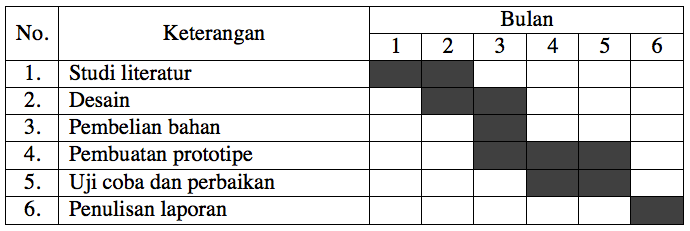
\includegraphics[width=13cm]{gambar/timeline}
\end{figure}

%-----------------------------------------------------------------
%Disini akhir masukan Bab
%-----------------------------------------------------------------

%-----------------------------------------------------------------
%Disini awal masukan untuk Daftar Pustaka
%-----------------------------------------------------------------
%%\nocite{Abel2010,Guerbas201350}
%%\bibliography{research-plan}
%%\bibliographystyle{plainnat}
\begin{thebibliography}{9}

\bibitem[satu(2013)]{satu01}
Annisa, Citra. 2010. Deteksi Tepi Citra Kanker Kulit Menggunakan Metode Laplacian Of Gaussian. Tugas akhir, tidak diterbitkan. Fakultas Sains dan Teknologi Universitas Islam Negeri Syarif Hidayatullah Jakarta

\bibitem[dua(2013)]{dua02}
Baskaraningrum, apriasih. 2011. Naïve Bayes Classifier Untuk Pengelompokan Keluarga Sejahtera Dan Keluarga Prasejahtera. Tugas akhir, tidak diterbitkan. Fakultas Ilmu Komputer Universitas Pembangunan Nasional “Veteran” Jakarta.

\bibitem[dua(2013)]{tiga03}
Desmita. 2007.Psikologi Perkembangan.Gramedia Pustaka Utama: Jakata

\bibitem[dua(2013)]{empat04}
Dusek, Jerome B. 1996. Adoloscent Development and Behavior. Prentice Hall: New Jersey

\bibitem[dua(2013)]{lima05}
Dwi, Andriyanto. 2013. Analisis Spam Filtering Pada Mail Server Dengan Metode Bayesian Chi-Square dan Naïve Bayes Classifier. Tugas akhir, tidak diterbitkan. Fakultas Matematika dan Ilmu Pengetahuan Alam Universitas Sebelas Maret Surakarta.

\bibitem[dua(2013)]{enam06}
Goleman, Daniel. 1996. Emotional Intelligence. Gramedia Pustaka Utaman: Jakarta.

\bibitem[dua(2013)]{delapan08}
Nafsiah, Siti. 2000. Professor Hembing Pemenang The Star Of Asia Award: Pertama Diasia Ke 3 Di Dunia. gema insane: Jakarta.

\bibitem[dua(2013)]{sembilan09}
Nursalam. 2003. Konsep  Dan Penerapan Metodologi Penenlitian Ilmu Keperawatan. Salemba Medika: Jakarta

\bibitem[dua(2013)]{sepuluh10}
Pahlevi, Rizal. 2010. Sistem Pendukung Keputusan Untuk Mendiagnosa Penyakit Tropis Yang Disebabkan Oleh Bakteri Menggunakan Metode Naïve Bayes Classifier. Tugas akhir, tidak diterbitkan. Fakultas Teknologi Industri Universitas Pembangunan Nasional “Veteran” Jakarta.

\bibitem[dua(2013)]{tigabelas13}
Hurlock, Elizabeth. 1998. Psikologi Perkembangan Suatu Pendekatan Sepanjang Rentang Kehidupan edisi kelima. Penerbit Erlangga. Jakarta.

\bibitem[dua(2013)]{delapanbelas18}
Sudjana. 1996. Metoda Statistika. Tarsito: Bandung

\bibitem[dua(2013)]{sembilanbelas19}
Warsiki, Endang,dkk. 2008. Insidens Kecemasan. http://www.kalbe.co.id/file/cdk/15 KecemasanPadaAnak Remaja.pdf

\end{thebibliography}
\addcontentsline{toc}{chapter}{DAFTAR PUSTAKA}
%-----------------------------------------------------------------
%Disini akhir masukan Daftar Pustaka
%-----------------------------------------------------------------

\end{document}